%%%%%%%%%%%%%%%%%%%%%%%%%%%%%%%%%%%%%%%%%
% Beamer Presentation
% LaTeX Template
% Version 1.0 (10/11/12)
%
% This template has been downloaded from:
% http://www.LaTeXTemplates.com
%
% License:
% CC BY-NC-SA 3.0 (http://creativecommons.org/licenses/by-nc-sa/3.0/)
%
%%%%%%%%%%%%%%%%%%%%%%%%%%%%%%%%%%%%%%%%%

%----------------------------------------------------------------------------------------
%	PACKAGES AND THEMES
%----------------------------------------------------------------------------------------

\documentclass{beamer}

\mode<presentation> {

% The Beamer class comes with a number of default slide themes
% which change the colors and layouts of slides. Below this is a list
% of all the themes, uncomment each in turn to see what they look like.

%\usetheme{default}
%\usetheme{AnnArbor}
%\usetheme{Antibes}
%\usetheme{Bergen}
%\usetheme{Berkeley}
%\usetheme{Berlin}
%\usetheme{Boadilla}
%\usetheme{CambridgeUS}
%\usetheme{Copenhagen}
%\usetheme{Darmstadt}
%\usetheme{Dresden}
%\usetheme{Frankfurt}
%\usetheme{Goettingen}
%\usetheme{Hannover}
%\usetheme{Ilmenau}
%\usetheme{JuanLesPins}
%\usetheme{Luebeck}
%\usetheme{Madrid}
%\usetheme{Malmoe}
%\usetheme{Marburg}
%\usetheme{Montpellier}
%\usetheme{PaloAlto}
%\usetheme{Pittsburgh}
\usetheme{Rochester}
%\usetheme{Singapore}
%\usetheme{Szeged}
%\usetheme{Warsaw}

% As well as themes, the Beamer class has a number of color themes
% for any slide theme. Uncomment each of these in turn to see how it
% changes the colors of your current slide theme.

%\usecolortheme{albatross}
%\usecolortheme{beaver}
%\usecolortheme{beetle}
%\usecolortheme{crane}
%\usecolortheme{dolphin}
%\usecolortheme{dove}
%\usecolortheme{fly}
%\usecolortheme{lily}
%\usecolortheme{orchid}
%\usecolortheme{rose}
%\usecolortheme{seagull}
\usecolortheme{seahorse}
%\usecolortheme{whale}
%\usecolortheme{wolverine}

%\setbeamertemplate{footline} % To remove the footer line in all slides uncomment this line
\setbeamertemplate{footline}[page number] % To replace the footer line in all slides with a simple slide count uncomment this line

\setbeamertemplate{navigation symbols}{} % To remove the navigation symbols from the bottom of all slides uncomment this line
}

\usepackage{graphicx} % Allows including images
\usepackage{booktabs} % Allows the use of \toprule, \midrule and \bottomrule in tables
\usepackage [T2A] {fontenc}   % Кириллица в PDF файле
\usepackage [utf8] {inputenc} % Кодировка текста: utf-8
\usepackage [russian] {babel} % Переносы, лигатуры


\usepackage{listings}
\usepackage{color}
\definecolor{lightgray}{rgb}{.9,.9,.9}
\definecolor{darkgray}{rgb}{.4,.4,.4}
\definecolor{purple}{rgb}{0.65, 0.12, 0.82}
\lstdefinelanguage{JavaScript}{
	keywords={break, case, catch, continue, debugger, default, delete, do, else, false, finally, for, function, if, in, instanceof, new, null, return, switch, this, throw, true, try, typeof, var, void, while, with, let, const},
	morecomment=[l]{//},
	morecomment=[s]{/*}{*/},
	morestring=[b]',
	morestring=[b]",
	ndkeywords={class, export, boolean, throw, implements, import, this,require, on},
	keywordstyle=\color{blue}\bfseries,
	ndkeywordstyle=\color{cyan}\bfseries,
	identifierstyle=\color{black},
	commentstyle=\color{purple}\ttfamily,
	stringstyle=\color{red}\ttfamily,
	sensitive=true
}

%----------------------------------------------------------------------------------------
%	TITLE PAGE
%----------------------------------------------------------------------------------------

\title[Выпускная квалификационная работа]{Разработка системы проведения опросов аудитории во время публичных выступлений} % The short title appears at the bottom of every slide, the full title is only on the title page
\subtitle{Выпускная квалификационная работа}
\author{Е.А.~Тактаров\\Научный руководитель ---  к.ф.-м.н., доцент Е.\,М.~Андреева} % Your name
\institute[ИММиКН] % Your institution as it will appear on the bottom of every slide, may be shorthand to save space
{
Южный Федеральный Университет\\
Институт математики, механики и компьютерных наук им. И.И. Воровича  \\ % Your institution for the title page
02.03.02 — Фундаментальная информатика и информационные технологии
}
\date{Ростов-на-Дону --- 2019} % Date, can be changed to a custom date

\begin{document}

\begin{frame}
\titlepage % Print the title page as the first slide
\end{frame}

\begin{frame}
\frametitle{Содержание} % Table of contents slide, comment this block out to remove it
\tableofcontents % Throughout your presentation, if you choose to use \section{} and \subsection{} commands, these will automatically be printed on this slide as an overview of your presentation
\end{frame}

%----------------------------------------------------------------------------------------
%	PRESENTATION SLIDES
%----------------------------------------------------------------------------------------

\section{Постановка задачи}
\begin{frame}
\frametitle{Постановка задачи}
Создать веб-сервис, отвечающий следующим требованиям:
\begin{itemize}
	\item Функция создания и проведения опросов. 
	\item Динамическое отображение результатов опроса на странице.
	\item Параллельное проведение нескольких опросов на одном развернутом веб-сервисе.
	\item Каждый опрос доступен по коротким ссылкам для голосования и просмотра результатов.
	\item Защита от вредоносного искажения результатов. 
	\item Открытый исходный код под свободной лицензией.
\end{itemize}
\end{frame}

%------------------------------------------------
\section{Обзор инструментов разработки}
\begin{frame}
\frametitle{Обзор инструментов разработки}
\begin{description}
	\item[Node.js] Программная платформа общего назначения для языка JavaScript. 
	\item[Express] Веб-фреймворк Node.js для создания серверной части веб-приложения.
	\item[WebSocket] Протокол связи поверх TCP-соединения, предназначенный для обмена сообщениями между браузером и веб-сервером в режиме реального времени.
	\item[Vue.Js] Веб-фреймворк для создания пользовательского интерфейса в браузерах.  
\end{description}
\end{frame}

%------------------------------------------------
\section{Аспекты Реализации}
%------------------------------------------------

\subsection{Структура веб-приложения}
\begin{frame}
\frametitle{Структура веб-приложения}
\begin{figure}
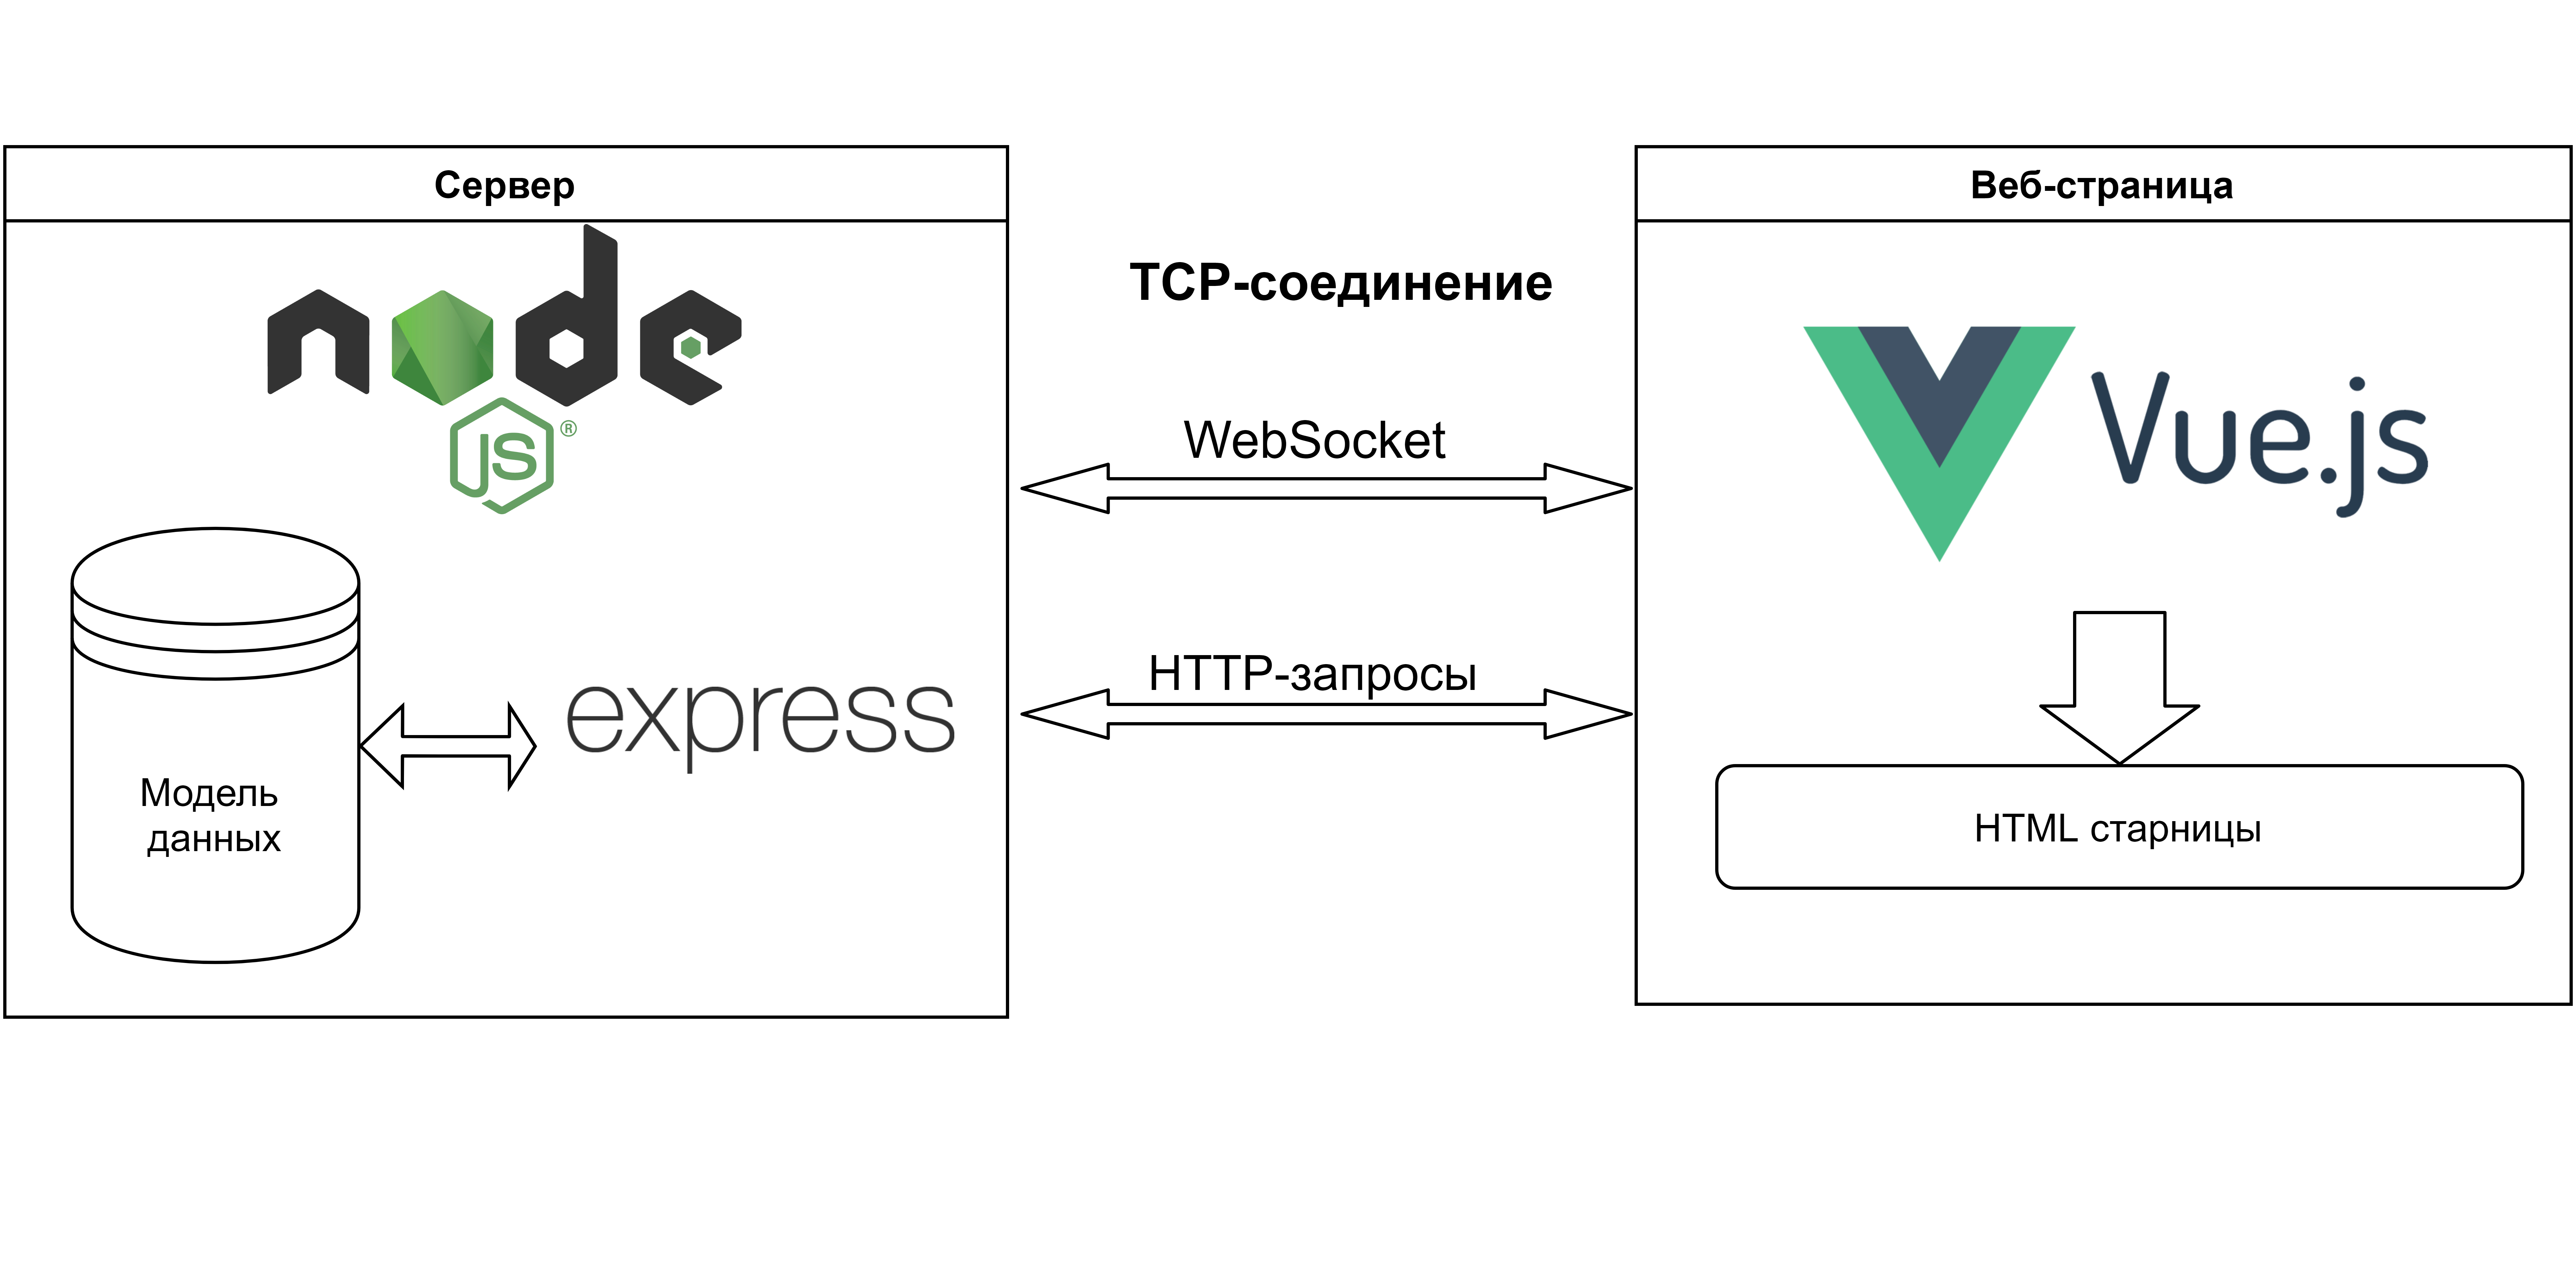
\includegraphics[width=\linewidth]{img/webdiagram.png}
\end{figure}
\end{frame}

%------------------------------------------------

\subsection{Веб-фреймворк Express}
\begin{frame}[fragile] % Need to use the fragile option when verbatim is used in the slide
\frametitle{Использование Express}

\begin{lstlisting}[language=JavaScript,columns=fullflexible]
router.get("/get_polled/:poll",function(req, res, next){
 let id = db.create_polling_session(req.params.poll);
 res.status(200).json({link:db.sessions[id].link});
});
\end{lstlisting}
\end{frame}
%------------------------------------------------

\begin{frame}
\frametitle{Требования к модели данных}
\begin{enumerate}
	\item В модели может существовать неограниченное количество параллельных сессий, которые могут перемещаться между своими опросами.
	\item Каждая сессия имеет две короткие ссылки для просмотра и участия в опросе. 
	\item Имея короткую ссылку, код должен уметь быстро переходить к данным о сессии, которой она принадлежит.
	\item Код должен быстро получать список пользователей, показывающих опрос или в нем участвующих.
	\item Пользователь может голосовать и перезагружать страницу неограниченное число раз, не вызывая подтасовку результатов.
	\item Модель должна быть устойчивой к добавлению новых видов взаимодействия пользователей с сервисом.
\end{enumerate}
\end{frame}

%------------------------------------------------

\subsection{Разработка модели данных}
\begin{frame}
\frametitle{Разработка модели данных}
	Особенности модели данных в приложении:
	\begin{itemize}
		\item JavaScript объект.
		\item Внутри рекурсивно списки, словари, объекты со свойствами и методами.
		 и экспортируется из него(всегда один экземпляр)
		\item Методы объектов инкапсулируют любое взаимодействие пользователей и модели.
		\item Каждый пользователь определяется объектом Websocket.
		\item События WebSocket'ов вызывают методы модели. 
		\item Модель определяется и инициализируется в отдельном модуле \textbf{database.js}.
		\item Модуль экспортирует один объект модели в любой точке кода(аналогично синглтону).
	\end{itemize}
\end{frame}




%------------------------------------------------

\subsection{Использование WebSocket}
\begin{frame}
\frametitle{Использование WebSocket}
	\begin{enumerate}
		\item Пакет \textbf{express-ws} добавляет в Express обработчики запросов на WebSocket-соединие.
		\item Клиент запрашивает соединение по URL:\\ \textbf{ws:[URL веб-сервиса]/ws/[короткая ссылка]}	  
		\item Данные отправляются в JSON. 
		\item Первое сообщение от клиента всегда содержит его идентификатор и тип сессии. 
		\item Если данные имеют неправильный формат или не совпадают с моделью данных, то сервер закрывает соединение.
	\end{enumerate}
\end{frame}

\begin{frame}
\frametitle{Алгоритм соединения через WebSocket}
\begin{figure}
	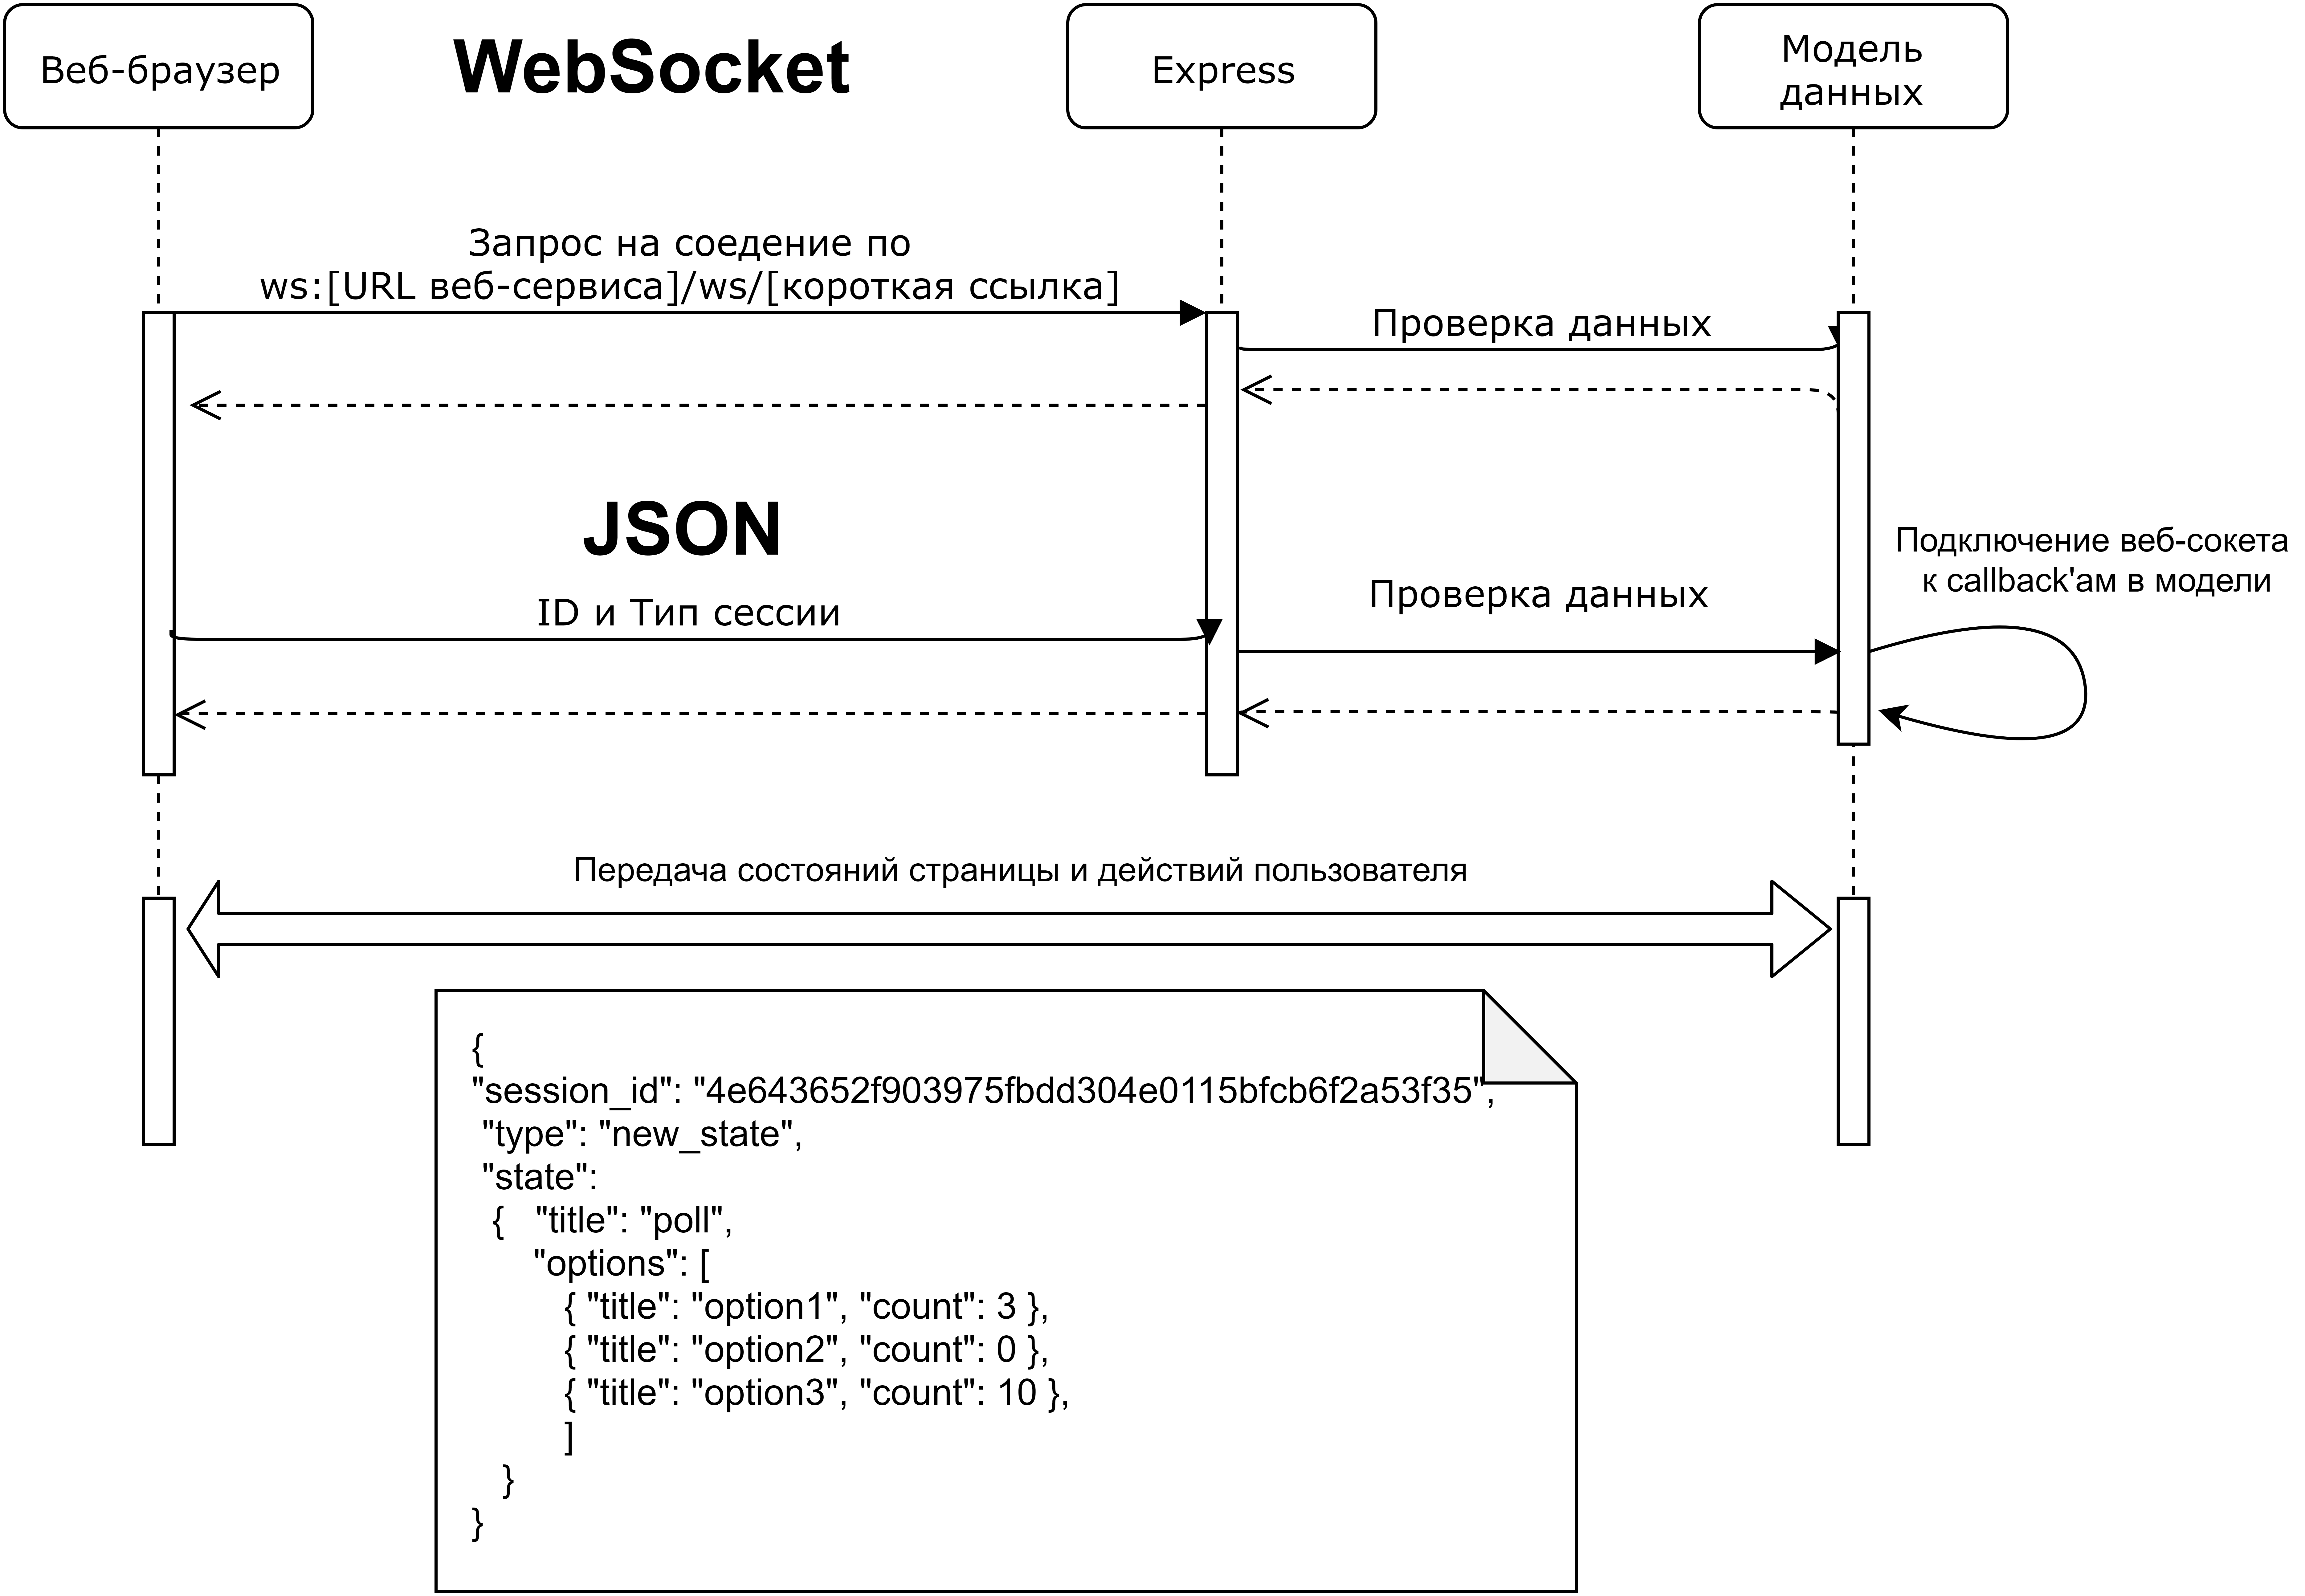
\includegraphics[width=\linewidth]{img/wsdiagram.png}
\end{figure}
\end{frame}

\subsection{Отложенный вызов с Debounce}
\begin{frame}
\frametitle{Проблема переполнения запросов}
\begin{figure}
	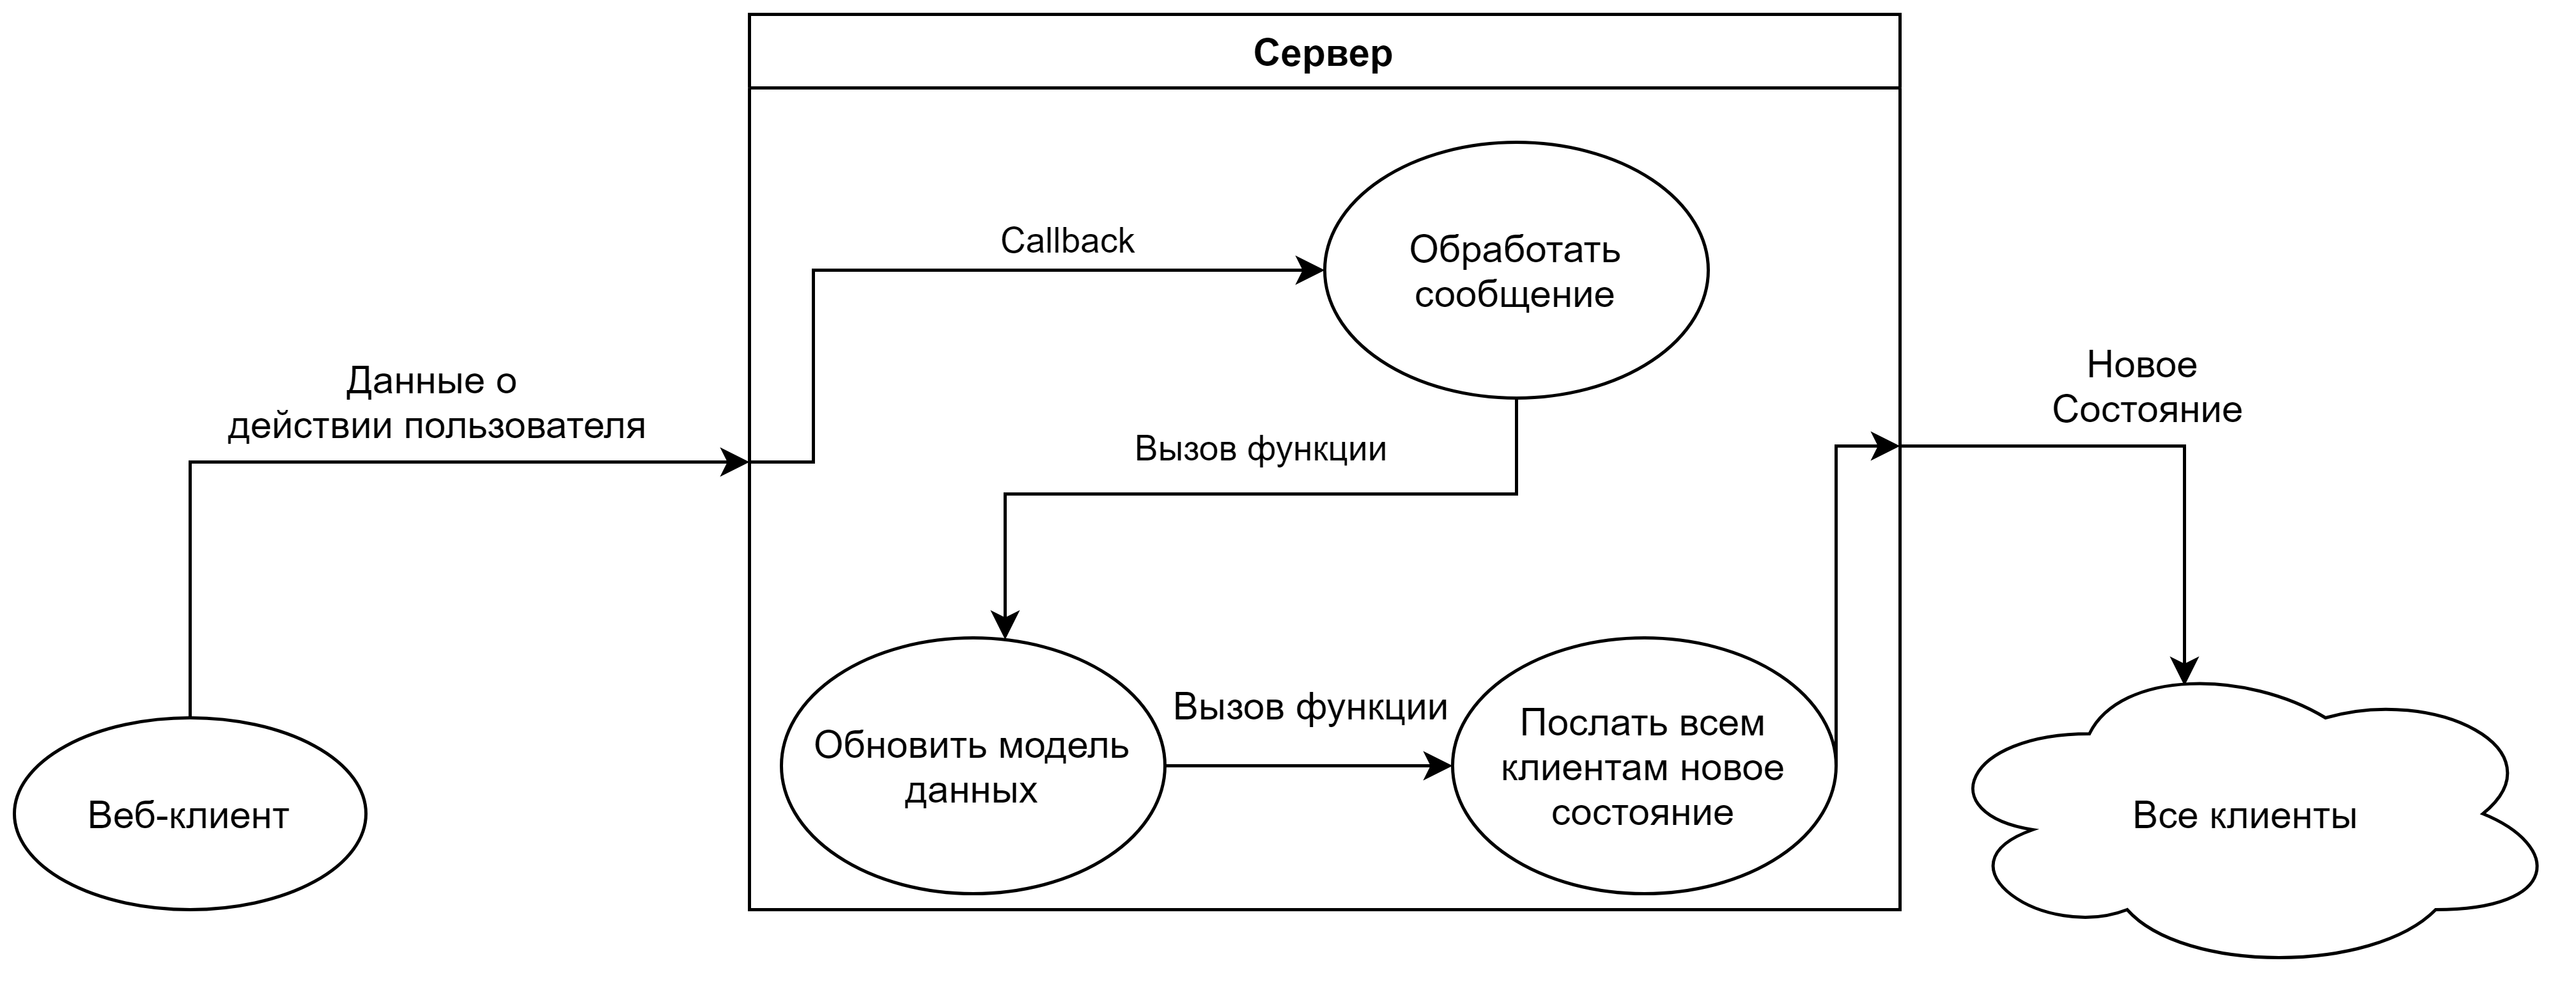
\includegraphics[width=\linewidth]{img/nodeb.png}
\end{figure}
	Что будет если 10 пользователей проголосуют одновременно?\\
	Каждому пользователю придет 10 сообщений с новым состоянием, и только последнее из них будет актуальным.  
\end{frame}

\begin{frame}
\frametitle{Использование отсроченного вызова}
\begin{description}
	\item[Debounce] пакет для Node.js, предоставляющий обертку для функций, которая откладывает их исполнение на указанный промежуток.
\end{description} 
	 \begin{figure}
	 	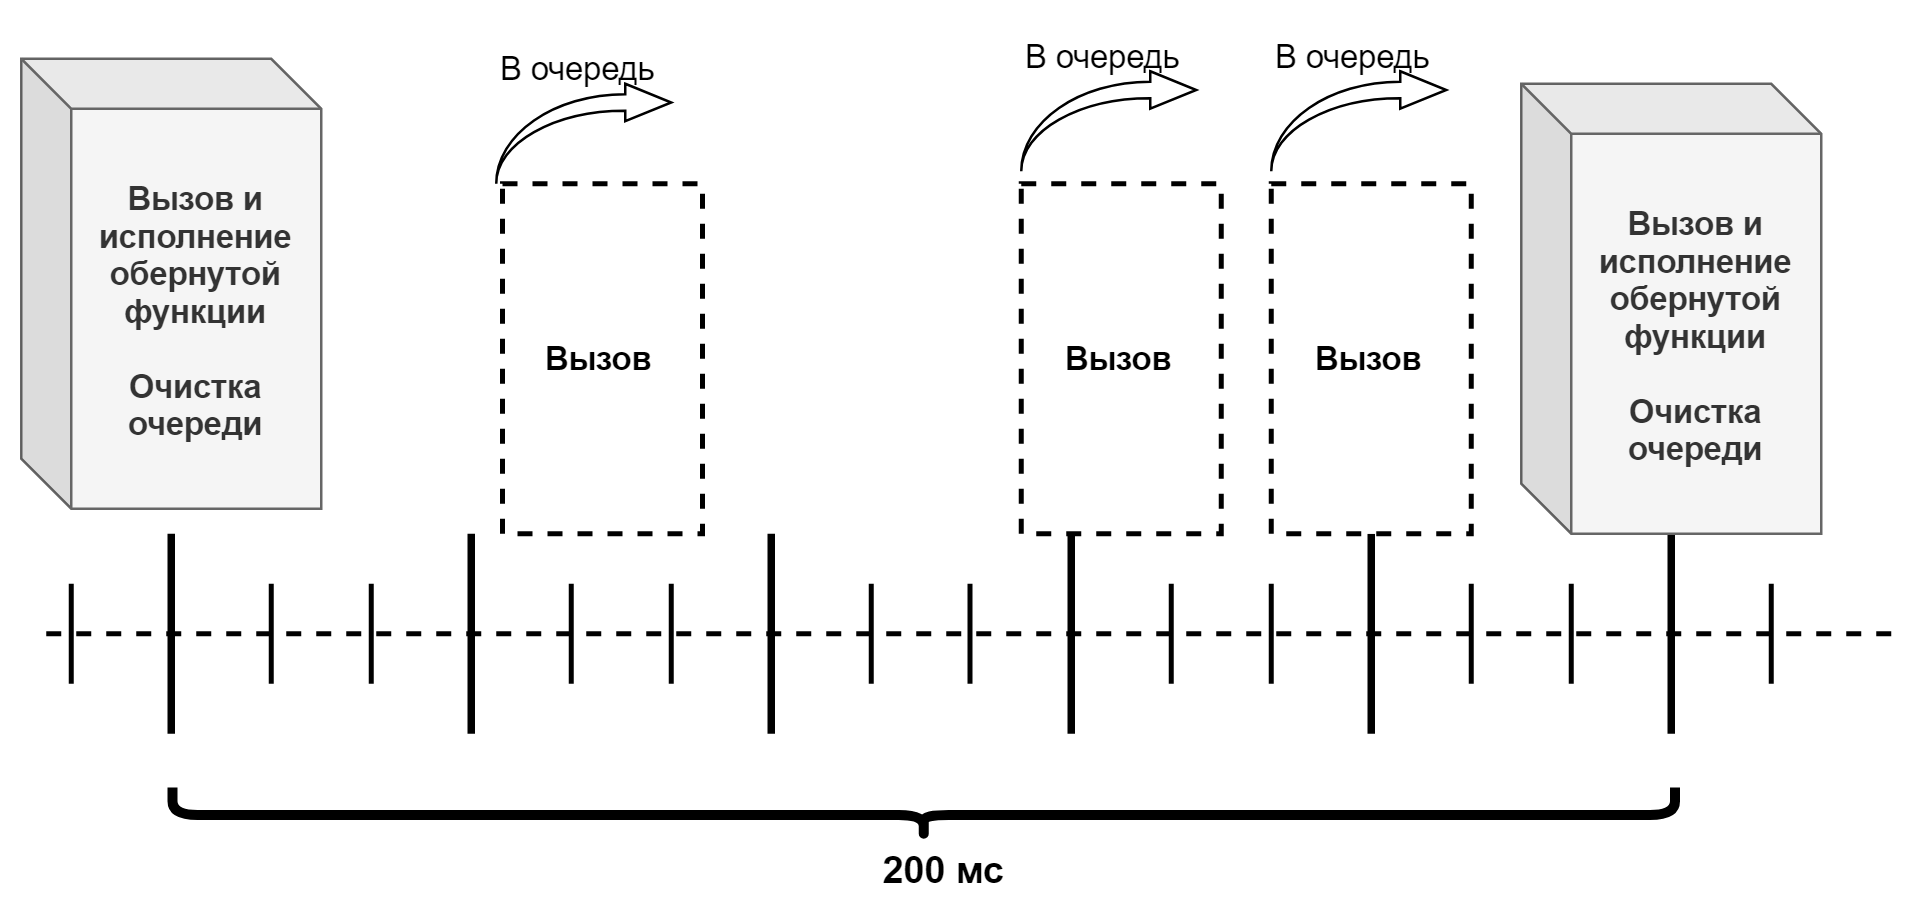
\includegraphics[width=\linewidth]{img/debounce.png}
	 \end{figure}
\end{frame}


\subsection{Интерфейс пользователя}
\begin{frame}
\frametitle{Устройство клиентской части}
\begin{figure}
	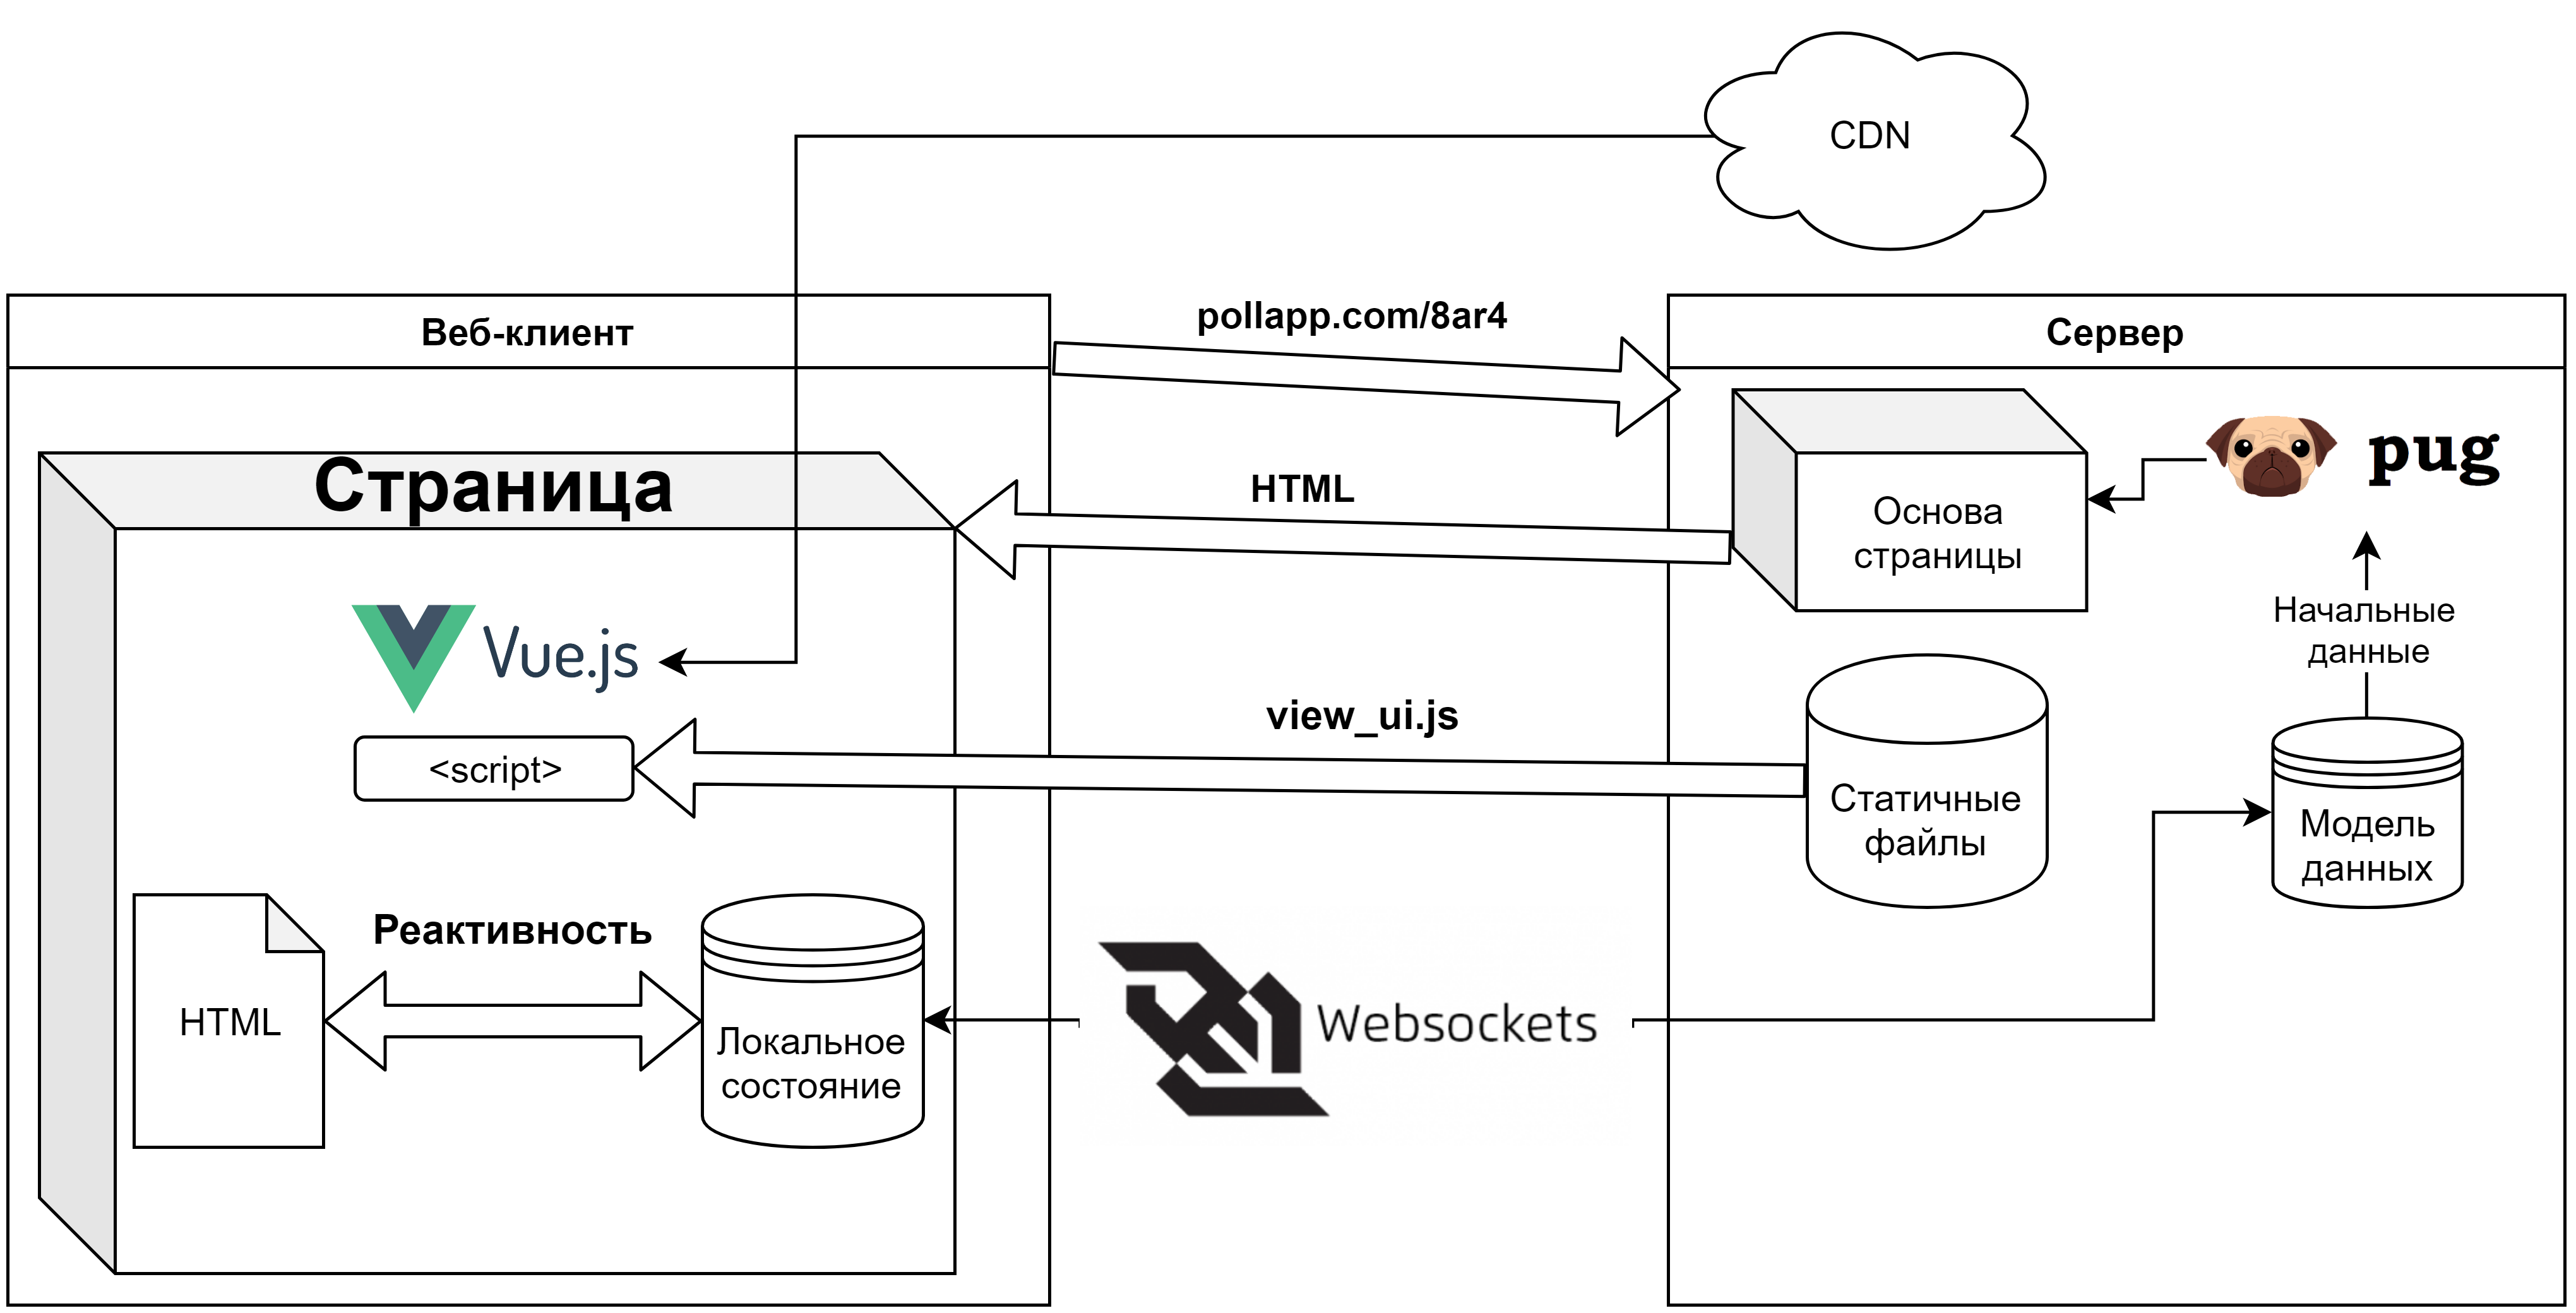
\includegraphics[width=\linewidth]{img/ui.png}
\end{figure}
\end{frame}

\begin{frame}
\frametitle{Со стороны пользователя}
\begin{columns}[c]

\column{.65\textwidth} % Left column and width
\begin{figure}
	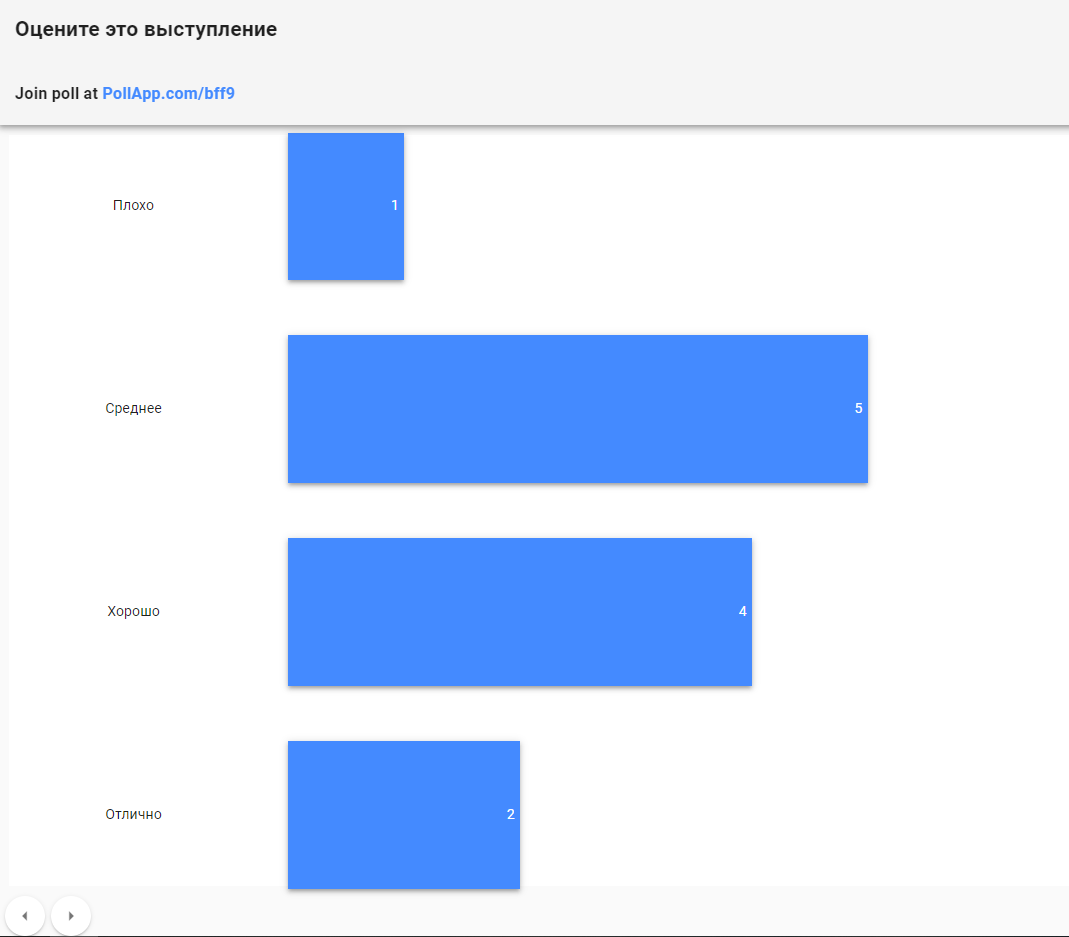
\includegraphics[width=\linewidth]{img/view.PNG}
\end{figure}


\column{.30\textwidth} % Left column and width
\begin{figure}
	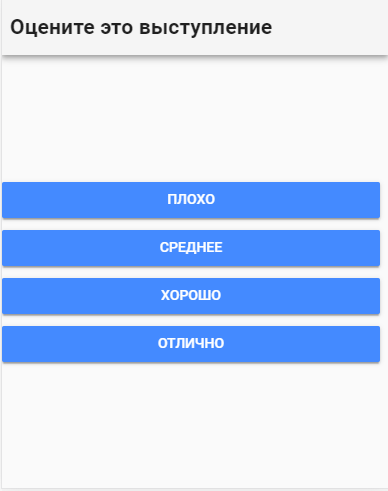
\includegraphics[width=\linewidth]{img/slave.PNG}
\end{figure}


\end{columns}
\end{frame}


\section{Результаты}
\begin{frame}
\frametitle{Полученные результаты}
	\begin{itemize}
		\item Веб-сервис позволяет создавать, проводить и управлять опросами.
		\item Одновременно может проводится неограниченное количество опросов.
		\item Пользователи могут сразу же поучаствовать в опросе со своего мобильного устройства, перейдя по короткой ссылке, указанной на экране опроса.
		\item Результаты голосования отображаются динамически на странице просмотра результатов.
		\item Реализована основная защита от вредоносного вмешательства в процесс опроса, не позволяющая испортить результаты или остановить ход опроса.
		\item Веб-сервис имеет открытые исходные коды на сайте \textbf{GitHub.com} и доступен для развертывания, использования и модификации по свободной лицензии MIT. 
	\end{itemize}   
\end{frame}





\end{document} 